\documentclass[10.7pt,]{article}

%Word count: up to 4000 words.
%Structured abstract: up to 250 words.
%Tables: up to 4.
%Figures: up to 6.
%References: unlimited.

\usepackage[letterpaper, margin=2.54cm, top=2.54cm]{geometry}
\usepackage[super,comma,sort&compress]{natbib}
\usepackage{lmodern}
\usepackage{authblk} % To add affiliations to authors
\usepackage{amssymb,amsmath}
\usepackage{wrapfig}
\usepackage{graphicx,grffile}
\usepackage[labelfont=bf,labelsep=period]{caption}
\usepackage{ifxetex,ifluatex}
\usepackage{multirow}
\usepackage[table]{xcolor}% http://ctan.org/pkg/xcolor

%\usepackage{fixltx2e} % provides \textsubscript
\ifnum 0\ifxetex 1\fi\ifluatex 1\fi=0 % if pdftex
  \usepackage[T1]{fontenc}
  \usepackage[utf8]{inputenc}
\else % if luatex or xelatex
  \ifxetex
    \usepackage{mathspec}
  \else
    \usepackage{fontspec}
  \fi
  \defaultfontfeatures{Ligatures=TeX,Scale=MatchLowercase}
    \setmainfont[]{Times New Roman}
    \setsansfont[]{Century Gothic}
    \setmonofont[Mapping=tex-ansi]{Consolas}
\fi
% use upquote if available, for straight quotes in verbatim environments
\IfFileExists{upquote.sty}{\usepackage{upquote}}{}
% use microtype if available
\IfFileExists{microtype.sty}{%
	\usepackage{microtype}
	\UseMicrotypeSet[protrusion]{basicmath} % disable protrusion for tt fonts
}{}

%\usepackage{lipsum} % for dummy text only REMOVE

\newtheorem{exm}{Example}

\usepackage{multirow}

%==============================
% Customization to make the output PDF 
% look similar to the MS Word version
%==============================
% To prevent hyphenation
\hyphenpenalty=10000
\exhyphenpenalty=10000

% To set the sections font size
\usepackage{sectsty}
\allsectionsfont{\fontsize{10}{10}\selectfont}
%\sectionfont{\fontsize{10}{10}\selectfont}
\subsectionfont{\itshape\bfseries\fontsize{10}{10}\selectfont}
\subsubsectionfont{\normalfont\itshape}

% No new line after subsubsection
\makeatletter
\renewcommand\subsubsection{\@startsection{subsubsection}{3}{\z@}%
	{-3.25ex\@plus -1ex \@minus -.2ex}%
    {-1.5ex \@plus -.2ex}% Formerly 1.5ex \@plus .2ex
    {\normalfont\itshape}}
\makeatother

\makeatletter % Reference list option change
\renewcommand\@biblabel[1]{#1.} % from [1] to 1
\makeatother %

% To set the doc title font
\usepackage{etoolbox}
\makeatletter
\patchcmd{\@maketitle}{\LARGE}{\bfseries\fontsize{15}{16}\selectfont}{}{}
\makeatother

% No page numbering
\pagenumbering{gobble}

\makeatletter
\def\maxwidth{\ifdim\Gin@nat@width>\linewidth\linewidth\else\Gin@nat@width\fi}
\def\maxheight{\ifdim\Gin@nat@height>\textheight\textheight\else\Gin@nat@height\fi}
\makeatother

% Scale images if necessary, so that they will not overflow the page
% margins by default, and it is still possible to overwrite the defaults
% using explicit options in \includegraphics[width, height, ...]{}
\setkeys{Gin}{width=\maxwidth,height=\maxheight,keepaspectratio}
\setlength{\parindent}{0pt}
\setlength{\parskip}{6pt plus 2pt minus 1pt}
\setlength{\emergencystretch}{3em}  % prevent overfull lines
\providecommand{\tightlist}{%
  \setlength{\itemsep}{0pt}\setlength{\parskip}{0pt}}
\setcounter{secnumdepth}{0}
% Redefines (sub)paragraphs to behave more like sections
\ifx\paragraph\undefined\else
\let\oldparagraph\paragraph
\renewcommand{\paragraph}[1]{\oldparagraph{#1}\mbox{}}
\fi
\ifx\subparagraph\undefined\else
\let\oldsubparagraph\subparagraph
\renewcommand{\subparagraph}[1]{\oldsubparagraph{#1}\mbox{}}
\fi
%==============================
\usepackage{hyperref}
\hypersetup{
	unicode=true,
	pdftitle={TableTidier: An UMLS powered data extraction tool},
	pdfauthor={Author One, Author Two, Author Three},
	pdfkeywords={keyword1, keyword2},
	pdfborder={0 0 0},
	breaklinks=true
}
\urlstyle{same}  % don't use monospace font for urls
%==============================

% reduce space between title and begining of page
\title{\vspace{-2em} TableTidier: An UMLS powered data extraction tool}
\author[ ]{\bf\fontsize{13}{14}\selectfont 
	Jesus A. Rodriguez Perez, PhD\textsuperscript{1}, 
	Elaine Butterly, PhD\textsuperscript{1}, 
	Lili Wei\textsuperscript{1}, 
	Avirup Chowdhury, MSc\textsuperscript{2}, 
	Peter Hanlon, MSc\textsuperscript{1},
	David McAllister, MD,\textsuperscript{1}
	\vspace{-.7em}
}
\affil[1]{\bf\fontsize{13}{14}\selectfont The University of Glasgow, UK}
\affil[2]{\bf\fontsize{13}{14}\selectfont Public Health Suffolk, Suffolk County Council, UK}
\date{} % add no date (by default date is added)

%==============================
\begin{document}
\maketitle
\vspace{-4em} %separation between the affiliations and abstract
%==============================

%==============================
\section{Abstract}\label{abstract}
%==============================
TableTidier is a software designed to assist in the clinical systematic review process. Systematic reviews is an essential exploratory procedure which focusses on the extraction of data from a sample of clinical documentation. Although many tools exist to assist in different areas of the systematic review process, no solution addresses the extraction of table data into a machine readable format effectively. Consequently, researchers are mostly left to extract data manually which poses obvious limitations in terms of the depth and breadth of their efforts. Our tool combines human-interaction, supervised classification methodologies, and web technologies to provide an end-to-end tool for data extraction in the context of clinical systematic reviews. In this paper, we study the effects of including UMLS-based features into our classification models, and its impact on the overall architecture of TableTidier. Our evaluation results demonstrate that including UMLS-based features consistently improves the performance of our classifiers, thus optimising the behaviour of TableTidier, which in turn reduces the labour needed by humans when undertaking a systematic review.

%==============================
\section{Introduction}\label{introduction}
%==============================

% I can introduce here actual tables. Good and Bad to motivate the semi-automatic extraction.

%%==============================
%\section{Background}\label{background}
%%==============================

Systematic reviews are highly influential in clinical decision making \cite{Murad125}. Following a pre-specified protocol, systematic reviews seek to obtain and extract all available relevant information on a  specific clinical question, with the largest and most influential reviews involving many hours of work for highly-trained researchers\cite{higgins2011cochrane}.

%(Chandler J, Cumpston M, Thomas J, Higgins JPT, Deeks JJ, Clarke MJ. Chapter I: Introduction. In: Higgins JPT, Thomas J, Chandler J, Cumpston M, Li T, Page MJ, Welch VA (editors). Cochrane Handbook for Systematic Reviews of Interventions version 6.0 (updated August 2019). Cochrane, 2019. Available from www.training.cochrane.org/handbook)

Consequently, a number of software tools\cite{systematicReviewTools} have been developed to assist researchers with the numerous labour-intensive tasks involved in systematic reviewing such as screening published papers for relevance, assessing studies for their risk of bias and extracting data from published results\cite{jonnalagadda2015automating, 10.1093/ije/dyv306, Tsafnat2014}. There are also a number of more generic software tools which may help with some aspects of systematic reviewing. For example, there are extensions available for programming languages commonly used in data analysis that provide functions for processing tabular data (E.g. Unpivotr\cite{unpivotr} and Databaker\cite{databaker}).

However, none of these tools are designed to assist in the (semi)-automatic extraction and standardisation of tabular results from published papers. Standardising such tables is not a trivial task; in the medical literature table design is highly idiosyncratic. Even where there are established reporting guidelines\cite{bian2011consort} there are no standards for table design, and aesthetic or branding considerations appear to be at least as important as consistency and accessibility. Indeed, features such as multi-level headers are common, and descriptions (labelling) of data-containing cells must often be inferred from ambiguous features such as formatting and the relative position of labels (Table \ref{tab:example}). Consequently, it requires both time and expertise to extract results from tables in the published literature and such data extraction is potentially error-prone.

In traditional systematic reviews of clinical trials, analyses might be based on only a few numbers for each trial. However, advances in the field of clinical trial meta-analysis mean that richer data are now needed \cite{phillippo_dias_elsada_ades_welton_2019} while systematic reviews of epidemiological studies often involve the extraction of large quantities of data covering a range of exposures and outcomes\cite{shah2015short}. Consequently, it has become more important to find ways to improve the efficiency of tabular data extraction. 

To address this issue, we developed TableTidier, a software tool which assists the conversion of tabular data to standard formats where each value is unambiguously labelled. Developed using medical journals articles reporting clinical trial findings, TableTidier uses a machine learning algorithm (a support vector machine) to estimate the table structure and content, based on the position, formatting and actual text of the table content.

We hypothesised that the use of the Unified Medical Language System (UMLS), which has been shown to improve such diverse tasks as information retrieval, as \cite{umlsPRFretrieval} and \cite{gurulingappa2016semi}, would improve the precision, accuracy and recall of this classification task.


%\subsection{Sklearn} Machine learning in python. Classifier families.


%==============================
\section{Research Problem}\label{methods}
%==============================
Extracting data from tables is very useful albeit a very challenging task. The main hurdle in automated table data extraction is need to preserve the relationship of data cells with respect to the headings that describe them.

%Why extracting tables? data not available in machine readable forms whichever the reason behind. 



\begin{table}[h!]
	\centering

\begin{tabular}{|c|c|c|}
	\hline 
	\multicolumn{3}{|c|}{Participants}  \\ 
	\hline 
	   & Placebo & Aspirin \\ 
	\hline 
Gender &200 & 300   \\ 
	\hline 
	 \hspace{1cm} Male & 90 & 160 \\ 
	\hline 
	 \hspace{1cm} Female & 110 & 140 \\ 
	\hline 
\end{tabular} 

	\caption{\label{tab:example} Example Table }
\end{table}

Consider Table \ref{tab:example} as an example. We can easily see that the data cell 200 is related to the Gender and Placebo headings. Similarly, 140 is related to the Female and Gender as well as Aspirin and Participants concepts. We can tell because the cells containing numbers are aligned with the headings, but also because of the indented formatting which aligns related concepts such as Gender to Male and Female. An example of the desired machine readable form is shown in Table \ref{tab:machine}.

\begin{table}[h!]
	\centering
	
	\begin{tabular}{|c|c|c|c|c|}
		\hline 

Participants & Placebo & Gender & & 200 \\
Participants & Placebo & Gender & Male & 90 \\
Participants & Placebo & Gender & Female & 110 \\
Participants & Aspirin & Gender & & 300 \\
Participants & Aspirin & Gender & Male & 160 \\
Participants & Aspirin & Gender & Female & 140 \\
		
		\hline 
	\end{tabular} 
	
	\caption{\label{tab:machine} Example Machine Readable Data }
\end{table}

These are visual cues that are easily interpreted by our brains, no matter how complex the tables are. Unfortunately, this behaviour is not so easily translated into algorithmic solutions. Additionally, we associate terms semantically, independently of their position in the table. Finally, although there are patterns, the data can be organised in any arbitrary way resulting in potentially infinite possible structures.

However, we believe there are basic elements that can be effectively exploited to enable semi-automated data extraction. These features can be derived from the position of concepts within the table and their textual formatting. Consequently we believe that by describing the structure of a table in terms of these features, we can use this description as a proxy to extracting the data from cells whilst keeping the relationships to the headings.

Furthermore, we believe that the inclusion of semantic features capable of linking concepts through its associated metadata can improve the fidelity of this semi-automated process. Since UMLS contains the vocabulary utilised in our domain, and is already organised as an ontology, it is a promising resource for our purposes. Thus we pose the following research question to drive our investigation: 

\begin{center}
\textit{\textbf{Can UMLS features enhance the performance and behaviour of the automated annotations provided by TableTidier?}}
\end{center}


%==============================
\section{System Architecture}\label{system-architecture}
%==============================

The TableTidier system is a web application composed by a number of modules organised within a classic Server / User Interface (UI) infrastructure.

\begin{figure}
	\centering
	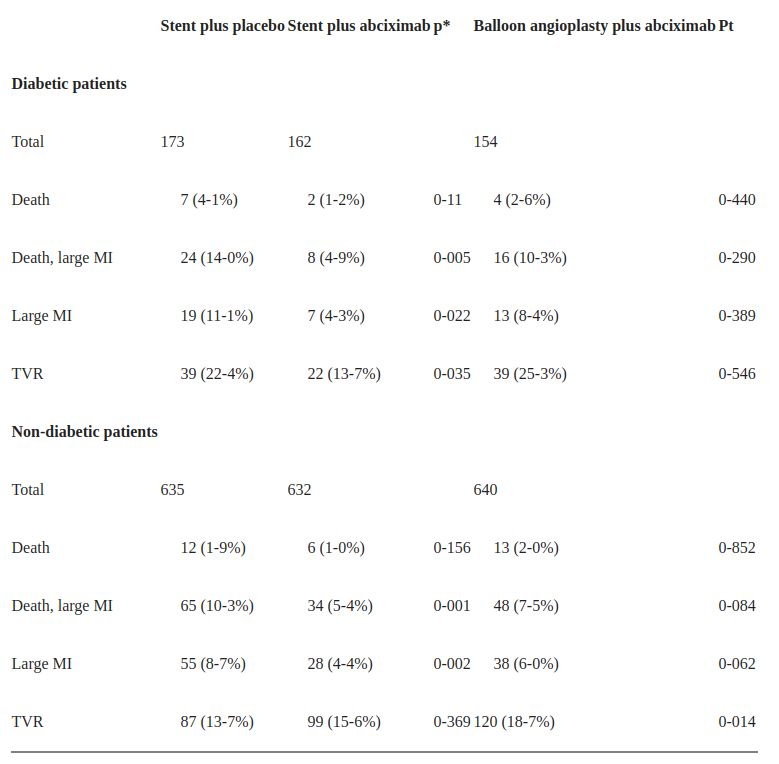
\includegraphics[width=0.7\linewidth]{screenshot003}
	\caption{TableTidier: Table to be annotated}
	\label{fig:annotator}
\end{figure}

%
%\begin{figure}
%	\centering
%	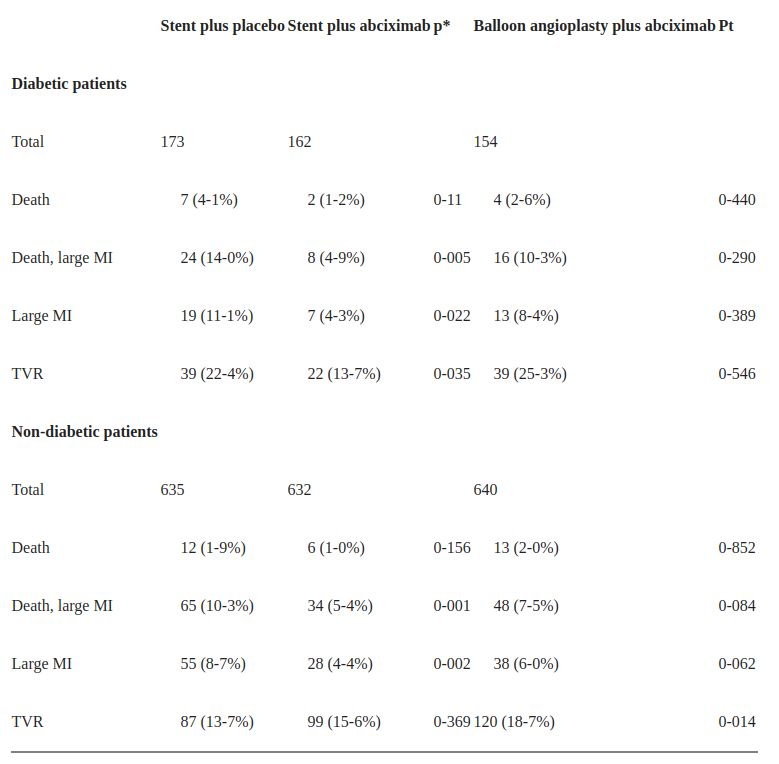
\includegraphics[width=0.7\linewidth]{screenshot003}
%	\caption{}
%	\label{fig:screenshot003}
%\end{figure}



\textbf{Server} written in Node.js combines all sub-modules that provide the data to the User Interface (UI):
	\begin{itemize}
		\item \textit{Automatic Annotation}: Predicts the structure of a table from the position and formatting of the different concepts.
		\item \textit{Data Extraction}: Module written in R which generates the machine readable data, from the table annotations.
		\item \textit{Database}: Provided by PostgreSQL, and holding data for results, user interactions, look-up tables, etc.
		\item \textit{MetaMap Interface}: Communicates with a ``dockerised''\footnote{https://metamap.nlm.nih.gov/DockerImage.shtml} version of MetaMap in order to assign concepts to the strings extracted from cells.
	\end{itemize}
	
\textbf{User Interface (UI)} coded in React.js, and comprises the following modules:
	\begin{itemize}
		\item \textit{Table Annotator}: Allows the users to manually and/or automatically annotate the structure of a table, for later data extraction.
		\item \textit{Live Table Editor}: Allows the user to edit tables on the fly, mostly used to fix OCR or transcription issues.
		\item \textit{Live Data Previewer}: Shows the data extracted on the fly, as users make changes to the table annotations.
		\item \textit{UMLS Concept Reviewer}: Allows to manually review, and edit the UMLS concepts automatically assigned to each of the strings in the tables.
	\end{itemize}	
	

\subsection{Data Extraction By Annotation}
Our approach to table data extraction involves a number of steps to be carried out by a user through TableTidier's UI:

\begin{enumerate}
	\item For every table to be annotated (Figure \ref{fig:annotator}), the user will be presented with two options (Figure \ref{fig:annotationPreview}):
	\begin{enumerate}
		\item[A.] Provide a manual ``annotation'' which describes the structure of the table in terms of its row/column content and format. Annotations are described by assigning a label to each relevant row and column which relates to its content, and by tagging any relevant formatting options as shown in Figure \ref{fig:annotationPreview}.
		\item[B.] Utilise the ``Automatic Annotator Module'' which attempts to simulate a human annotation (The focus of this study), and edit the annotation if needed.
	\end{enumerate}	
	\item In both cases, the ``Live Data Previewer'' (Figure \ref{fig:annotationPreview}) attempts to extract the data given the previous annotation, and display a preview of the machine readable format.
	\item Once all tables are annotated, the user can obtain all extracted data in a machine readable format directly from the interface.
	\item[\textit{Optional 1}] If any problems are encountered, the user can manually edit the table with the Live Table Editor.
	\item[\textit{Optional 2}] UMLS concepts will be automatically assigned to each of the table concepts, and the user may decide to review and/or later them in the UMLS Concept Reviewer
\end{enumerate}


\begin{figure}
	\centering
	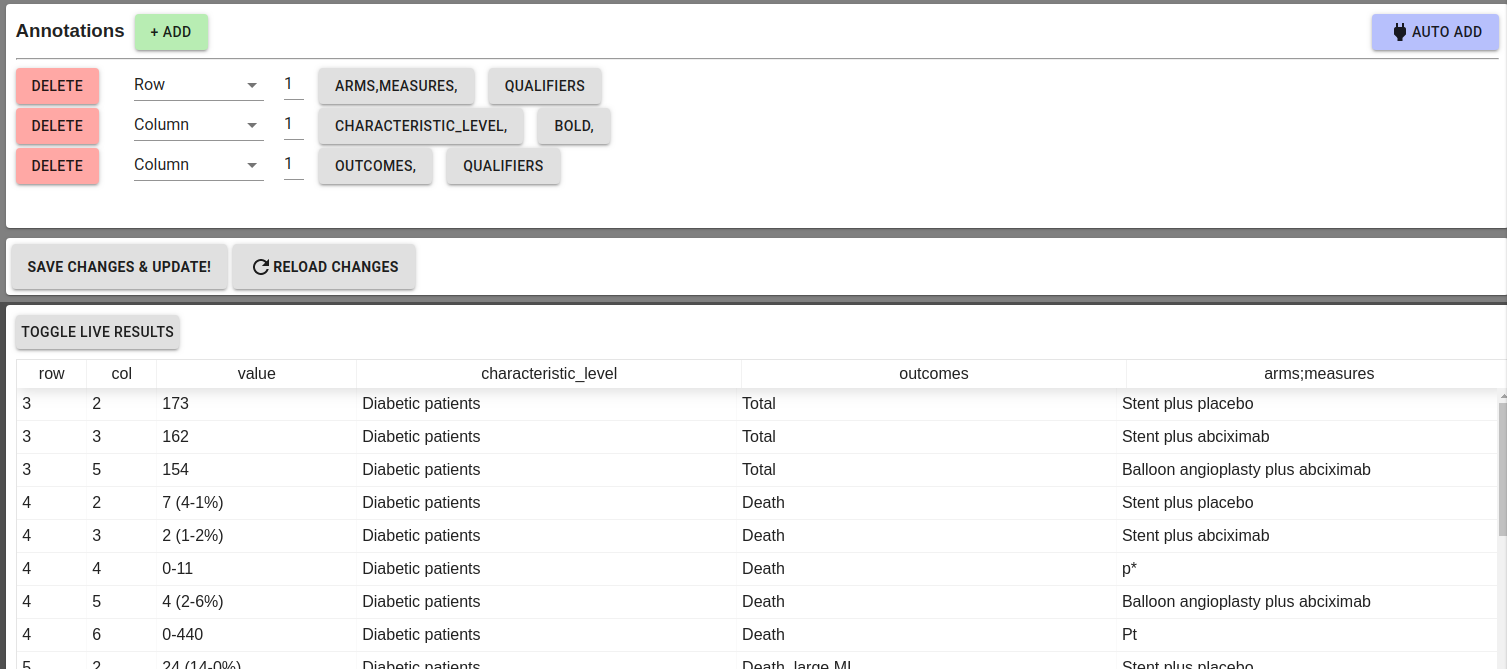
\includegraphics[width=\linewidth]{screenshot004}
	\caption{TableTidier: Annotation and Live preview example}
	\label{fig:annotationPreview}
\end{figure}

%==============================
\subsection{Data sources}\label{data-sources}
%==============================
	
	
\textbf{Tables Dataset} : The 1900 tables in our dataset originate from the "denominator trials" shown in Figure 1 of our recent publication \cite{Hanlon2019}. Briefly, eligible trials were registered via the US Clinical Trials Register (clinicaltriasl.gov), started on or after 1st January 1990, were phase 3 or 4, recruited at least 300 participants, had an upper age of at elast 60 years and evaluated drugs for a selected set of chronic conditions.

\textbf{UMLS} : The UMLS \cite{10.1093/nar/gkh061}, or Unified Medical Language System, is a set of medical ontologies and interfacing software, which allows the interaction between many biomedical vocabularies, thus enabling the interoperability of computer systems. Its Metathesaurus includes popular vocabularies such as ICD-10, MeSH and SNOMED, linked together by means of a semantic ontology which associates concepts through semantic relationships.

\textbf{MetaMap: } MetaMap \cite{10.1136/jamia.2009.002733} is software developed by Dr. Alan (Lan) Aronson at the National Library of Medicine (NLM) which allows the processing of text utilising NLP\footnote{Natural Language Processing} techniques, and its subsequent linkage to the UMLS metathesaurus. We make extensive use of MetaMap in our evaluation to derive our UMLS-based features, in particular CUIs\footnote{Concept Unique Ids} and SemanticTypes\cite{semtypes}.

%==============================
\subsection{Features}\label{features}
%==============================

\begin{enumerate}
	\item \textbf{pos\_start}: Whether the concept appears in the first row of the table.
	\item \textbf{pos\_middle}: Whether the concept appears between the first and last rows of the table.
	\item \textbf{pos\_end}: Whether the concept appears in the last row of the table.
	\item \textbf{inRow}: Whether the concept appears in a row containing headings 
	\item \textbf{inCol}: Whether the concept appears in a column of headings 
	\item \textbf{is\_bold}: Whether the concept is formatted as bold
	\item \textbf{is\_italic}: Whether the concept is formatted as bold
	\item \textbf{is\_indent}: Whether the concept is formatted as indented
	\item \textbf{is\_empty\_row}: Whether the concept is in the only populated cell of its row
	\item \textbf{is\_empty\_row\_p}: Whether the concept appears in a row, where the only other populated cell contains a ``P value''
	\item \textbf{semanticTypes}: The UMLS semantic groups assigned by MetaMap to the text on each cell. (\textit{e.g. ``inpo'' semanticType code for ``Injury or Poisoning''})
	\item \textbf{cuis}: The Concept Unique Identifiers (CUIs) assigned by MetaMap to each of the text strings in the table cells. (e.g. C0001779 which represents the concept ``Age'' )
%	\item label: Whether the is formatted as bold
\end{enumerate}

\textbf{Note:} Multiple CUIs and semanticTypes can be associated with a single string of text.

%==============================
\section{Evaluation}\label{evaluation}
%==============================
In this section we introduce the specifications of our evaluation dataset, evaluation metrics and the classifiers utilised in this study.
%
%In our evaluation we are set to measure the performance differences arising from the use of UMLS features with respect to the absence of them. 
%
%To this end we utilise a number of classifiers and compare them by means of standard evaluation metrics commonly used in the context of information retrieval.

\subsection{Dataset}

Our evaluation dataset comprises manual annotations on the 1900 tables mentioned above. We performed a feature extraction over all concepts belonging to either annotated rows or columns, and all features described in the previous Section. This was done on the basis of the original table label strings, prior to identification of any CUIs from metamap.

We then mapped each string to metamap, resulting in a matrix with 40729 rows and 6550 features, as each possible CUI and semanticType is assigned a column.

The features introduced in the Section above, were utilised to produce four different feature sets to thoroughly test our classifiers:

\begin{itemize}
	\item \textbf{Basic}: Set without UMLS features (Features 1-10).
	\item \textbf{UMLS-SemTypes}: Same as Basic, but adding the \textbf{semanticTypes} feature from UMLS (Features 1-11).
	\item \textbf{UMLS-CUIs}: Same as Basic, but adding the \textbf{cuis} feature from UMLS (Features 1-10, 12).
	\item \textbf{UMLS-Full}: Includes all features (Features 1-12)
\end{itemize}

The dataset was split into training (70\%) and testing (30\%) stratifying on the target labels to be classified (eg arms, characteristic\_level, characteristic\_name, measures, other, outcomes, p-interaction, time/period), which ensured all labels are well represented\footnote{https://scikit-learn.org/stable/modules/generated/sklearn.model\_selection.train\_test\_split.html}. 

%\begin{figure}
%	\centering
%	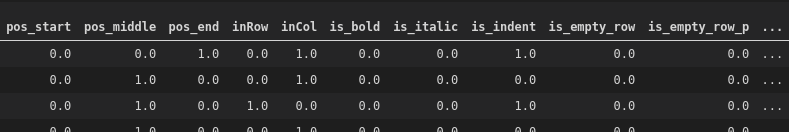
\includegraphics[width=0.7\linewidth]{screenshot005}
%	\caption{Evaluation Dataset Example.}
%	\label{fig:screenshot005}
%\end{figure}


\subsection{Classifiers}
To test whether any additional benefits from adding UMLS features to the text are dependent on a particular modelling approach, we repeated the modelling using a number of commonly used classifiers based on diverse methodologies:


\begin{itemize}
	\item Neural Network: Multi-layer Perceptron (\textbf{MLP})
	\item Naive-Bayes: \textbf{MultinomialNB}
	\item Logistic Regression: \textbf{LogReg}
	\item Tree: \textbf{RandomForest}
	\item Ensemble: \textbf{AdaBoost}
\end{itemize}

%==============================
\subsection{Evaluation Metrics} \label{measures}
%==============================
We used a range of evaluation metrics across for each of these comparisons, precision, recall, F1-Score, accuracy Macro\_Avg and weighted\_Avg:

\begin{itemize}
	\item \textbf{Precision}: Also referred to as positive predictive value, the number of correctly assigned cells as a proportion of the total number of cells assigned to that label  % $ tp / (tp + fp) $
	\item \textbf{Recall}: Also referred to as sensitivity, the number of correctly assigned cells as a proportion of the total number of cells which should have been assigned to that label  %$ tp / (tp + fn) $, also referred to as sensitivity
	\item \textbf{F1-Score}: A metric that combines precision and recall given a mixing parameter $ F $. $ F1 $ in particular gives the same importance to Precision and Recall, thus $F=1$
%	\textbf{WHY DOESNT IT LIE BETWEEN PRECISION AND RECALL FOR ROW 1}
	\item \textbf{Accuracy}: Is the proportion of correctly assigned labels from all test samples
	\item \textbf{Macro\_avg}: Standard average over results across all labels
	\item \textbf{Weighted\_avg}: Average weighted over the number of existing samples for each of the labels to be predicted
\end{itemize}

--- Seems \cite{urbano2019statistical} that ttest is appropriate for IR metrics given their experiments ---



%For the automatic annotation task we introduce an adapted version of Precision, namely Table Precision (TP). TP is defined as the rate of matching between the human annotation and the automatic annotation provided by our system.

%==============================
\section{Discussion}\label{results}
%==============================
Table \ref{tab:Sum-all} shows summary results for all classifiers with four different feature sets, \textit{Basic}, \textit{UMLS-SemTypes}, \textit{UMLS-CUIs} and \textit{UMLS-Full}. The results were averaged over the results obtained for each label to be classified. In other words, the evaluation metrics were computed as in Table \ref{tab:RF-basic} for all labels (e.g. arms, measures, outcomes...), and we utilised the average over results for all labels (e.g. macro\_avg) to produce the summary results in Table \ref{tab:Sum-all}. Accuracy is an exception as it does not relate to any labels and thus was computed over the whole test set.

\begin{table}
	\centering
	\begin{tabular}{|c|c|c|c|c|c|}

\hline
\multirow{2}{*}{\textbf{Features} }	& \multicolumn{5}{c|}{\textbf{Metrics Averaged Over All Target Labels (Macro\_avg)}} \\
\cline{2-6}
 &		\textbf{Classifier} & \textbf{Precision} &  \textbf{Recall} & \textbf{F1-Score} & \textbf{Accuracy (12k)}\\
		\hline 
		\hline 
		
\multirow{5}{*}{ \textit{Basic} } & MLP & \textbf{0.46} & \textbf{0.23} & \textbf{0.19} & \textbf{0.59} \\ 
	\cline{2-6}
		& MultinomialNB & 0.22 & 0.22 & 0.17 & 0.57 \\ 
	\cline{2-6}
		& LogReg & 0.21 & 0.22 & 0.18 & \textbf{0.59} \\
	\cline{2-6}
		& RandomForest & 0.39 & \textbf{0.23} & \textbf{0.19} & \textbf{0.59} \\ 
	\cline{2-6}
		& AdaBoost & 0.14 & 0.21 & 0.17 & 0.58 \\

		
		\hline
		\hline

\multirow{5}{*}{ \textit{UMLS-SemTypes}  } & MLP & 0.52 & 0.42 & 0.45 & 0.64 \\
	\cline{2-6}
	& MultinomialNB & 0.34 & 0.29 & 0.28 & 0.60 \\
	\cline{2-6}
	& LogReg & 0.42 & 0.29 & 0.29 & 0.62 \\
	\cline{2-6}
	& RandomForest & \textbf{0.56} & \textbf{0.43} & \textbf{0.46} & \textbf{0.65} \\
	\cline{2-6}
	& AdaBoost & 0.33 & 0.23 & 0.22 & 0.57 \\
	
	\hline
	\hline

\multirow{5}{*}{ \textit{UMLS-CUIs}  } & MLP & 0.61 & \textbf{0.51} & \textbf{0.53} & \textbf{0.67} \\  
\cline{2-6}
& MultinomialNB & 0.42 & 0.35 & 0.36 & 0.62 \\
\cline{2-6}
& LogReg & 0.59 & 0.39 & 0.42 & 0.66 \\
\cline{2-6}
& RandomForest & \textbf{0.65} & \textbf{0.51} & 0.52 & \textbf{0.67} \\
\cline{2-6}
& AdaBoost & 0.23 & 0.24 & 0.20 & 0.59 \\

		
\hline
\hline

\multirow{5}{*}{ \textit{UMLS-Full}  } & MLP & \textbf{0.59} & 0.52 & \textbf{0.54} & \textbf{0.67} \\
\cline{2-6}
& MultinomialNB & 0.42 & 0.36 & 0.36 & 0.62 \\
\cline{2-6}
& LogReg & 0.58 & 0.39 & 0.42 & 0.66 \\
\cline{2-6}
& RandomForest & \textbf{0.59} & 0.50 & 0.53 & \textbf{0.67} \\
\cline{2-6}
& AdaBoost & 0.23 & 0.26 & 0.21 & 0.59 \\
\hline

\hline

		
	\end{tabular} 
	\caption{\label{tab:Sum-all} Summary statistics for all feature sets and classifiers  }
\end{table}

There was substantial variation in the performance across the classifiers. Nonetheless, all five showed improved results for all evaluation metrics on the addition of UMLS features.

There was an improvement in all precision (and therefore by definition recall) with no loss of accuracy. UMLS semantic types \cite{semtypes} alone improved precision, recall and accuracy compared to basic feature set. However, there was a larger improvement with the addition of CUIs. %\textbf{WHICH ALSO CONTAIN INFORMATION ON ...}].
There was no evidence of further improvement when both sematic types and CUIs were combined in the modelling (\textit{UMLS-Full}).

Since the improvement was similar across all classifier types, we used the RandomForest classifier as an example to formally test whether the changes in accuracy with addition of UMLS features were statistically significant. Table \ref{tab:stat-diff}, as expected, is consistent with the findings in Table \ref{tab:Sum-all}. There was statistically significant evidence (at the conventional $ p < 0.05 $) level of improved performance on adding UMLS semantic types or CUIs to the basic feature set, and better performance of CUIs compared to semantic types, but little evidence for using both CUI and semantic types. 
%
%\textbf{I DONT THINK A PAIRED T-TEST, WHICH IS A TEST FOR CONTINUOUS DATA F IS VALID. I THINK YOU COULD USE MCNEMAR'S TEST FOR PAIRED PROPORTIONS https://www.rdocumentation.org/packages/stats/versions/3.6.2/topics/mcnemar.test. -  IT IS MUCH MORE CONVENTIONAL TO COMPARE THE AREA UNDER THE ROC CURVES, AT LEAST IN MEDICINE https://www.rdocumentation.org/packages/pROC/versions/1.16.1/topics/roc.test THIS IS REALLY EASY TO RUN IN R WITH THE DATA SET-UP THE WAY YOU HAVE. IT ALSO GIVES YOU ANOTEHR STATISTIC TO INCLUDE AS THE RESULTS ARE A BIT THIN}

\begin{table}
	\centering
	\setlength{\tabcolsep}{0.5em} % for the horizontal padding
	{\renewcommand{\arraystretch}{1.2}% for the vertical padding
	\begin{tabular}{c|c|c|c|c}
		%	\hline 
		\cellcolor{black!50} & \textbf{Basic} & \textbf{UMLS-SemTypes}  & \textbf{UMLS-CUIs}  & \textbf{UMLS-Full} \\ 
		\hline 
		\textbf{Basic} &  \cellcolor{black!50} & $1.47^{-61}$ & $9.91^{-77}$ & $7.67^{-90}$ \\ 
		\hline 
		\textbf{UMLS-SemTypes} & $1.47^{-61}$ & \cellcolor{black!50} & $6.25^{-6}$ & $3.25^{-11}$ \\ 
		\hline 
		\textbf{UMLS-CUIs} & $9.91^{-77}$ & $6.25^{-6}$ & \cellcolor{black!50} & $0.01$ \\ 
		\hline 
		\textbf{UMLS-Full} & $7.67^{-90}$ & $3.25^{-11}$ & $0.01$ & \cellcolor{black!50} \\ 
		%	\hline 
	\end{tabular}
	}
	
	\caption{ \label{tab:stat-diff} Paired T-Test p-values comparing RandomForest classification runs }
\end{table}


\begin{table}
	\centering
	\begin{tabular}{c|c|c|c|c}

		
		&\textbf{Precision} &  \textbf{Recall} & \textbf{F1-Score} & \textbf{Samples} \\
		\hline 
		\hline 
		arms & 0.53 & 0.81 & 0.64 & 1217 \\
		\hline
		characteristic\_level & 0.60 & 0.95 & 0.73 & 6466 \\
		\hline
		characteristic\_name & 0.37 & 0.01 & 0.01 & 2636 \\
		\hline
		measures & 0.72 & 0.04 & 0.08 & 754 \\
		\hline
		other & 0.73 & 0.05 & 0.09 & 167 \\
		\hline
		outcomes & 0.12 & 0.00 & 0.00 & 895 \\
		\hline
		p-interaction & 0.00 & 0.00 & 0.00 & 10 \\
		\hline
		time/period & 0.00 & 0.00 & 0.00 & 74 \\
		\hline
		\hline
		
		macro\_avg & 0.39 & 0.23 & 0.19 & \multirow{2}{*}{12219.00}  \\
		\cline{1-4}
		weighted\_avg & 0.52 & 0.59 & 0.46 & \\
		\hline
		\hline	
		accuracy&\multicolumn{4}{c}{0.58} \\ 
		\hline
	\end{tabular} 
	\caption{\label{tab:RF-basic} RandomForest classifier results, basic features (No UMLS)  }
\end{table}


\begin{table}
	\centering
	\begin{tabular}{c|c|c|c|c}
		
		&\textbf{Precision} &  \textbf{Recall} & \textbf{F1-Score} & \textbf{Samples} \\
		\hline 
		\hline 
		
		arms & 0.82 & 0.85 & 0.83 & 1217 \\
		\hline
		characteristic\_level & 0.68 & 0.86 & 0.76 & 6466 \\
		\hline
		characteristic\_name & 0.46 & 0.22 & 0.30 & 2636 \\
		\hline
		measures & 0.72 & 0.62 & 0.66 & 754 \\
		\hline
		other & 0.60 & 0.32 & 0.42 & 167 \\
		\hline
		outcomes & 0.68 & 0.53 & 0.60 & 895 \\
		\hline
		p-interaction & 0.20 & 0.10 & 0.13 & 10 \\
		\hline
		time/period & 0.55 & 0.57 & 0.56 & 74 \\
		\hline
		\hline
		macro\_avg & 0.59 & 0.51 & 0.53 & \multirow{2}{*}{12219}  \\
		\cline{1-4}
		weighted\_avg & 0.65 & 0.67 & 0.64 & \\
		\hline
		\hline	
		accuracy & \multicolumn{4}{c}{0.66} \\ 
		\hline
	\end{tabular} 
	\caption{\label{tab:RF-all} RandomForest classifier results with Full UMLS features enabled }
\end{table}



% Random forest best overall

% Achieves comparable performance when using only semtypes to the full

%\begin{table}
	\centering
	\begin{tabular}{c|c|c|c|c}
		
		& \textbf{Precision} &  \textbf{Recall} & \textbf{F1-Score} & \textbf{Samples} \\
		\hline 
		\hline 
		
		arms & 0.54 & 0.81 & 0.65 & 1207 \\ 
		\hline
		characteristic\_level & 0.59 & 0.95 & 0.73 & 6396 \\ 
		\hline
		characteristic\_name & 0.57 & 0.00 & 0.01 & 2677 \\ 
		\hline
		measures & 0.59 & 0.03 & 0.05 & 746 \\ 
		\hline
		other & 0.83 & 0.03 & 0.06 & 169 \\ 
		\hline
		outcomes & 0.50 & 0.01 & 0.01 & 933 \\ 
		\hline
		p-interaction & 0.00 & 0.00 & 0.00 & 12 \\ 
		\hline
		time/period & 0.00 & 0.00 & 0.00 & 79 \\ 
		
		\hline
		\hline
		
		macro\_avg & 0.45 & 0.23 & 0.19 & \multirow{2}{*}{12219}  \\ 
		\cline{1-4}
		weighted\_avg & 0.57  &  0.58  &  0.45 &  \\
		\hline
		\hline	
		accuracy & \multicolumn{4}{c}{0.64} \\ 
		\hline
	\end{tabular} 
	\caption{\label{tab:MLP-semantic} MultiLayer Perceptron (MLP), results with Basic feature set }
\end{table}

Tables \ref{tab:RF-basic} and \ref{tab:RF-all} show similar metrics as Table \ref{tab:Sum-all}, solely for the \textit{RandomForests} classifier, but broken down by the different label types. The performance improves for all features when utilising UMLS features as evidenced across all metrics, with the exception of the ``other'' category. Since the ``other'' label was poorly defined by the manual reviewers, it is difficult to interpret this finding. For some labels, ``p-interaction'' and ``time/period'' there were striking improvements in performance when UMLS features were included.

We can conclude that utilising UMLS features significantly improves performance of our classifier, which in turn should positively affect the automatic annotation module of TableTidier. This improvement translates directly to less manual labour for the users, thus reducing the time involved in data extraction in tasks such as systematic reviews.

%

%
%
%
%
%\begin{table}
%	\centering
%	\begin{tabular}{|c|c|c|c|c|}
%		\hline 
%		&\textbf{Precision} &  \textbf{Recall} & \textbf{F1-Score} & \textbf{Samples} \\
%		\hline 
%		\hline 
%		
%		arms&0.82 & 0.80 & 0.81&1207 \\ 
%		\hline
%		characteristic\_level&0.69 & 0.79 & 0.74&6396 \\ 
%		\hline
%		characteristic\_name&0.43 & 0.31 & 0.36&2677 \\ 
%		\hline
%		measures&0.68 & 0.67 & 0.67&746 \\ 
%		\hline
%		other&0.46 & 0.31 & 0.37&169 \\ 
%		\hline
%		outcomes&0.64 & 0.55 & 0.59&933 \\ 
%		\hline
%		p-interaction&0.00&0.00&0.00&12 \\ 
%		\hline
%		time/period&0.61 & 0.51 & 0.55&79 \\ 
%		
%		\hline
%		\hline
%		
%		macro\_avg&0.54 & 0.49 & 0.51&\multirow{2}{*}{12219}  \\ 
%		\cline{1-4}
%		weighted\_avg&0.64 & 0.65 & 0.64& \\
%		\hline
%		\hline	
%		accuracy&\multicolumn{4}{c|}{0.65} \\ 
%		\hline
%	\end{tabular} 
%	\caption{\label{tab:MLP-semantic} MultiLayer Perceptron (MLP), results with UMLS CUIS }
%\end{table}
%\begin{table}
%	\centering
%	\begin{tabular}{|c|c|c|c|c|}
%		\hline 
%		&\textbf{Precision} &  \textbf{Recall} & \textbf{F1-Score} & \textbf{Samples} \\
%		\hline 
%		\hline 
%		
%		arms&0.81&0.80&0.80&1207 \\ 
%		\hline
%		characteristic\_level&0.65&0.88&0.75&6396 \\ 
%		\hline
%		characteristic\_name&0.42&0.17&0.24&2677 \\ 
%		\hline
%		measures&0.65&0.53&0.59&746 \\ 
%		\hline
%		other&0.54&0.18&0.27&169 \\ 
%		\hline
%		outcomes&0.63&0.37&0.47&933 \\ 
%		\hline
%		p-interaction&0.00&0.00&0.00&12 \\ 
%		\hline
%		time/period&0.38&0.18&0.24&79 \\ 
%		
%		\hline
%		\hline
%		
%		macro\_avg&0.51&0.39&0.42&\multirow{2}{*}{12219}  \\ 
%		\cline{1-4}
%		weighted\_avg&0.61 & 0.64 & 0.60& \\
%		\hline
%		\hline	
%		accuracy&\multicolumn{4}{c|}{0.64} \\ 
%		\hline
%	\end{tabular} 
%	\caption{\label{tab:MLP-semantic} MultiLayer Perceptron (MLP), results with UMLS SemanticType }
%\end{table}
%
%
%
%
%\begin{table}
%	\centering
%	\begin{tabular}{|c|c|c|c|c|}
%		\hline 
%		&\textbf{Precision} &  \textbf{Recall} & \textbf{F1-Score} & \textbf{Samples} \\
%		\hline 
%		\hline 
%		
%		arms&0.82 & 0.80 & 0.81&1207 \\ 
%		\hline
%		characteristic\_level&0.69 & 0.79 & 0.74&6396 \\ 
%		\hline
%		characteristic\_name&0.43 & 0.31 & 0.36&2677 \\ 
%		\hline
%		measures&0.68 & 0.67 & 0.67&746 \\ 
%		\hline
%		other&0.46 & 0.31 & 0.37&169 \\ 
%		\hline
%		outcomes&0.64 & 0.55 & 0.59&933 \\ 
%		\hline
%		p-interaction&0.00&0.00&0.00&12 \\ 
%		\hline
%		time/period&0.61 & 0.51 & 0.55&79 \\ 
%		
%		\hline
%		\hline
%		
%		macro\_avg&0.54 & 0.49 & 0.51&\multirow{2}{*}{12219}  \\ 
%		\cline{1-4}
%		weighted\_avg&0.64 & 0.65 & 0.64& \\
%		\hline
%		\hline	
%		accuracy&\multicolumn{4}{c|}{0.65} \\ 
%		\hline
%	\end{tabular} 
%	\caption{\label{tab:MLP-semantic} MultiLayer Perceptron (MLP), results with UMLS CUIS }
%\end{table}

%
%%==============================
%\section{}\label{discussion}
%%==============================
%
%This Table \ref{tab:stat-diff} speaks about something

%==============================
\section{Conclusion}\label{conclusion}
%==============================

Systematic reviews are highly influential in clinical decision making, and increasingly require the extraction of large quantities of data from tables published in scholarly journals, which is a challenging and labour-intensive task. We found that adding UMLS features to software designed to aid this task markedly improved precision, recall and accuracy. 

We built a system that exploits the structure of tables in order to convert them into a machine readable format, in a semi-automated manner, by means of a classifier. The basic software relied upon the position of concepts within the tables, as well as the existence of formatting cues. However, we also found that adding UMLS-based features into the classifier - CUI codes and SemTypes assigned by MetaMap which represent features with different levels of specificity - markedly improved prediction. Importantly, this finding was robust to the choice of classifier (eg random forest, neural network), making it unlikely that a better machine-learning algorithm, or more skill in fitting such a model would, without the rich contextual knowledge embedded in UMLS and MetaMap, have been unlikely to achieve similar levels of performance.
%
%\textbf{THESE EXPLANATIONS NEED TO GO IN MUCH EARLIER [CUI is a unique concept identifier, and SemType refers to the semantic family it belongs to]}


MetaMap is a complex software with many options and functions. We elected to use the out-of-the-box defaults, and alternative options may have led to better or worse performance. However, our decision to do so does mean that over-fitting is a highly unlikely explanation for the improved performance we observed, since we made a very small number of modelling choices (i.e. the basic model versus two different sources of information from Metamap using default settings.)

%\textbf{would be good to throw in some discussion here about to expand on my point below}

A strength of this study includes the fact that the allocation of labels by the manual reviewers was done blinded to (indeed prior to) the mapping of strings to UMLS concepts. However, there are number of weaknesses in our study. First, we only examined tables for one subject area, clinical trials, and we do not know if the use of UMLS will increase performance similarly in closely related fields such as pharmaco-epidemiology, or in moderately-related fields such as genetic, biomarker, clinical and social epidemiology. Nonetheless, the influential role of clinical trials within evidence-based medicine mean that our findings are of some importance despite our selection of a single field.

Mapping strings from published tables of clinical trial reports to UMLS using MetaMap resulted in dramatic improvements in our ability to automatically classify labels. This was consistent across the type of label (eg arm, time, outcome) and across the choice of classifier (eg random forest, neural network). Thus the integration of UMLS and MetaMap into our (and perhaps other's) tools have the potential to reduce the manual work involved in conducting systematic reviews.


%
%data extraction system
%
%powered by UMLS classifier
%
%Which in turn powers an automatic annotator
%
%conclusion better performance with UMLS features
%
%Users more efficient than before. capable of more complexity and/or time saving


%==============================
\section{Acknowledgements}\label{acknowledgements}
%==============================
We would like to thank Hebe Shedden and Yifan Shen for their help in compiling a substantial part of the training data used in this study. Furthermore, we would like to thank Wellcome Trust for funding this project.

%Remember to acknowledge your funding institution\ldots

%==============================
\bibliographystyle{vancouver}
\bibliography{literature}
%==============================

\end{document}